\IEEEPARstart
{H}{aptic} feedback is an essential component in the robotic master systems because it allows to the user to perceive the interaction of the slave with the surrounding environment. 
In particular haptic feedback can be divided in kinesthetic and cutaneous feedback. This two types of stimuli are very different from each other, kinesthetic feedback acts on muscles, joints and tendons, instead cutaneous feedback acts on the skin.
Cutaneous feedback has been a great source of interest in the last years for the researchers that looking for a valid alternative to force feedback, a type of kinesthetic feedback used in a lot of robotics solutions. Unfortunately in many areas this kind of stimuli is not applicable because it is a source of instability for the system. For example in the commercial solutions of teleoperated surgical robots is not possible to use a force feedback because a little error could be very dangerous for the patient.
\par
% Cuteneous feedback in general
In \cite{pacchierotti2012two} the authors built a system that provide the sense of weight on the finger. They used a servo motor that pulls three wires with the purpose to provide a compression of the finger, in this way they reproduced the contact of the slave system tools with the environment.
\par
% Vibratory feedback
More recently the researchers were focused on the vibratory feedback. This kind of stimuli was used in \cite{pacchierotti2014teleoperation} combined with kinesthetic feedback in teleoperation of steerable flexible needle to provide different type of feedback for different type of interaction.
The experimental results show that this system is very helpful for the clinician and it greatly reduces the error.
\par
% Combination of feedbacks with the vibratory one
In \cite{pacchierotti2015cutaneous} vibratory feedback was used for palpation in robotic surgery. A BioTac tactile sensor was mounted on a Da Vinci robot and a custom 3-DoF cutaneous feedBack device was built to act vibratory feedback on the master controller (Fig.2). This experiment proves that the palpation of internal tissue is possible to do with a minimally invasive surgical procedure.
\par
Inspired by the great success of vibratory feedback in the last years this paper presents another way to exploit it. 
The system consists of master controller and slave robot, the master controller is responsible for the user hand mapping and for the applying of the vibratory feedback on the same hand, instead the slave robot is characterised by an robotic hand that follows the user hand movements and when it interacts with the environment it sends to the glove weared by the user the values measured by the sensors on the robotic hand. This setup allows to do a wide range of experiments to evaluate the goodness of this kind of feedback.
% The paper is organized as follow...
%% Qui bisogna dire cosa viene descritto nei successivi capitoli


%\begin{figure}
%  \centering
%  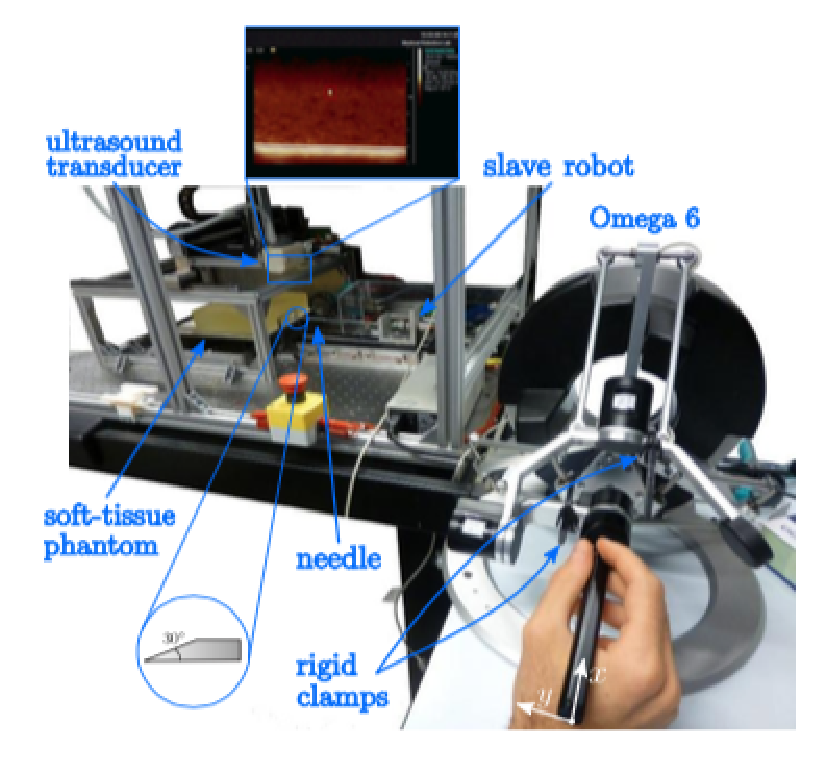
\includegraphics[width = 0.9\columnwidth]{img/img1.eps}
%  \caption{Simulation results for the network.}
%  % \label{fig_trajectory}
%\end{figure}
%
%\begin{figure}
%  \centering
%  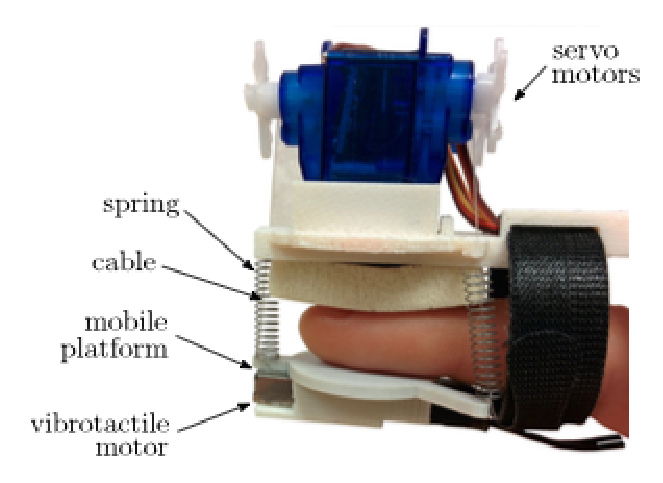
\includegraphics[width = 0.9\columnwidth]{img/vibrotactiledevice.eps}
%  \caption{custom 3-DoF cutaneous feedback device}
%  % \label{fig_trajectory}
%\end{figure}